% Created 2016-02-05 Fri 21:47
% Indented LaTeX compiler: pdflatex
\documentclass[11pt]{article}
\usepackage[utf8]{inputenc}
\usepackage[T1]{fontenc}
\usepackage{graphicx}
\usepackage{grffile}
\usepackage{longtable}
\usepackage{wrapfig}
\usepackage{rotating}
\usepackage[normalem]{ulem}
\usepackage{amsmath}
\usepackage{textcomp}
\usepackage{amssymb}
\usepackage{capt-of}
\usepackage{hyperref}
\usepackage[hmargin=2.5cm,vmargin=2.5cm]{geometry}
\usepackage{mathpazo} \usepackage{paralist}
\usepackage{enumitem}
\usepackage{amsmath}
\usepackage{tikz}
\usetikzlibrary{shapes, positioning}
\setlength{\parskip}{0.5cm} \setlength{\parindent}{0cm}
\usepackage{lscape}
\usepackage{booktabs}
\hypersetup{colorlinks=true,linkcolor=blue,urlcolor=blue}
\author{John Henderson}
\date{2016 February (TCRUG meetup)}
\title{R + Org-mode = awesome!\\\medskip
\large Org-mode for science, reproducible research, organization}
\hypersetup{
 pdfauthor={John Henderson},
 pdftitle={R + Org-mode = awesome!},
 pdfkeywords={},
 pdfsubject={},
 pdfcreator={Emacs 24.5.1 (Org mode 8.3.3)}, 
 pdflang={English}}
\begin{document}

\maketitle


\section*{Background}
\label{sec:orgheadline1}

I work in product development at 3M. I'd \emph{like} to say my job consists
of coming up with ideas, trying things out, collecting and analyzing
data, using that knowledge for the next iteration, and eventually launching a finished
product. Those steps are certainly involved, but my life \emph{also} involves a hefty dose of
meetings, emails and phone calls, keeping track of various bits of information, compliance
courses, lots of todos/deadlines, volunteering activities, and other general miscellany.

It might not seem like a big deal, but as I tried various applications, I simply found
that I disliked storing notes, todos, contacts, data, code, etc. in separate formats and
locations. To date, I'm unaware of another solution that lets you do what Org-mode can do, which is
what I'd like to introduce here!
\begin{itemize}
\item General notes/information organization
\item Todos and planning (scheuling/deadlines/states)
\item Export to html, pdf (\LaTeX{}/Beamer), markdown, open document formats, and more
\item Numerous supported programming languages (R, python, bash, gnuplot, among others)
\item Citations/references
\item Inserting code results (both blocks and inline code)
\item Inserting images into exported documents
\item Even using code to print out Org-mode syntax, thus allowing programmatically generated
document structures (say a headline per some repeated systematic analysis)
\end{itemize}

These features extremely well for those working in technical/scientific fields, as well as
enabling literate programming and reproducible research. Just so it's clear, I'm certainly
not the first to discover or present this. There's an excellent article about Org-mode for
reproducible research written by various Org-mode contributors, as well as an
example of such work by Thomas Dye.\footnote{Schulte, Eric; Davison, Dan; Dye, Thomas S; Dominik, Carsten. \emph{A Multi-Language Computing Environment for Literate Programming and Reproducible Research}. 
Journal of Statistical Software. \url{http://www.jstatsoft.org/article/view/v046i03}} \textsuperscript{,}\,\footnote{Dye, Thomas S. \emph{Structure and Growth of the Leeward Kohala Field System: An
Analysis with Directed Graphs}. PlosONE. \url{http://journals.plos.org/plosone/article?id=10.1371/journal.pone.0102431}}

\section*{This document}
\label{sec:orgheadline2}

I wrote this to serve as a quick demo of Org-mode features for a live demonstration at the
\href{http://www.meetup.com/twincitiesrug/}{Twin Cities R User Group} (TCRUG). I re-created a minimal version of my \texttt{\textasciitilde{}/.emacs} config
file in an effort to make it easier for newer users to dive in. From there, I simply
created some quick examples and notes on some of the various Org-mode features. This file
is meant to serve as a living Org-mode tutorial. You can see the code, options, and
markup that relate to each feature and actually try them out. And don't worry, there's a
backup version, \texttt{demo-backup.org}, so feel free to play around! 

\section*{Basic features I use}
\label{sec:orgheadline8}

Shortcuts are defined in Emacs like this: \texttt{C-x} (Ctrl+x) and \texttt{M-x} (alt+x). They can be
strung together and interspersed with other text like this: \texttt{M-x org-mode RET} would mean
"press alt+x, type 'org-mode' and press the enter key."

The short list of \emph{super} basic emacs shortcuts you might be lost without:
\begin{itemize}
\item \texttt{C-x C-f}: open a file
\item \texttt{C-x C-s}: save file
\item \texttt{C-g}: when there's a message in that little line way at the bottom (called the
minibuffer) and you can't make it shut up/stop/go away
\item \texttt{C-x u}: undo
\end{itemize}

Headings are defined by one or more asterisks at the start of a line in Org-mode:
\subsection*{Sub-heading 1}
\label{sec:orgheadline3}
\subsection*{Sub-heading 2}
\label{sec:orgheadline4}
\subsection*{Sub-heading 3}
\label{sec:orgheadline5}

lists
\begin{itemize}
\item item 1
\item item 2
\item item 3
\end{itemize}

You can move headings/items up and down with \texttt{M-up/down}; you can promote/demote with
\texttt{M-left/right}. \texttt{Alt-RET} starts a new heading/list of the same type you're cursor is
currently on. \texttt{Ctrl-RET} starts a new heading at the same level of the one you're in.

You can insert todos using a heading and any defined keyword (in this case, \texttt{next}, \texttt{todo},
\texttt{wait}, \texttt{cancelled}, and \texttt{done}):

\subsection*{project 1}
\label{sec:orgheadline6}

\subsection*{project 2}
\label{sec:orgheadline7}

\section*{Agenda}
\label{sec:orgheadline9}

The easiest way to use agenda to start is on this file. Go before the first headline and
do \texttt{C-u M-x org-agenda-set-restriction-lock}.\footnote{You can also set files Org-mode agenda via commands listed \href{http://orgmode.org/manual/Agenda-files.html#Agenda-files}{here}.} This will set agenda mode to only look at
this file. After that, run it with \texttt{C-c a}.

You can choose from the various options which bring up default views (like filters). You
can also write your own to show, for example, a dashboard of only today's action items.

The \texttt{m} option is quite handy for matching defined tags or dates (if you know what you're
looking for). I use \texttt{C-a s} (search) far more. It brings up a list of hits for a keyword
for each instance in your agenda files.

\section*{Some extra stuff}
\label{sec:orgheadline11}

Sometimes I get test data from a lab assistant who uses various file naming schemes. I've
come to love \href{http://www.emacswiki.org/emacs/Sunrise_Commander}{Sunrise Commander} to edit these quickly in Emacs with things like \texttt{regex} and
rectangle operations.

Speaking of rectangles, these can be really handy in tables and whatnot.

\begin{center}
\begin{tabular}{lllr}
\toprule
\textbf{Mfg} & \textbf{Type} & \textbf{Grade} & \textbf{Yield \%}\\
\midrule
Dow & PP & A & 5\\
Dow & PE & B & 7\\
Dow & PE & C & 7\\
Lyondell & LDPE & 1 & 13\\
Lyondell & LDPE & 2 & 14\\
Lyondell & LDPE & 3 & 16\\
\bottomrule
\end{tabular}
\end{center}


Org-mode also has a neat interface for entering things quickly called \texttt{capture}. I have it
bound to \texttt{C-c c}, which brings up some options for what I want to capture. It's really
nice for quickly entering a bunch of todos, which are filed into a location of your
choosing.

You can track your time with clocking by going to a headline and doing \texttt{C-c C-x i/o} to
clock in/out. You can insert a clock table with \texttt{M-x org-clock-report}. Update it with
\texttt{C-c C-c}.

\begin{table}[htb]
\caption{Clock summary at \textit{[2016-02-05 Fri 21:35]}}
\centering
\begin{tabular}{lrr}
\toprule
Headline & Time & \\
\midrule
\textbf{Total time} & \textbf{4:41} & \\
\midrule
todos & 4:41 & \\
\hspace*{1.0em}done create content &  & 1:43\\
\hspace*{1.0em}done migrate/anonymize example data set &  & 0:24\\
\hspace*{1.0em}todo get beamer/slidify/reveal working &  & 1:07\\
\hspace*{1.0em}todo verify local setup file/libraries &  & 1:00\\
\hspace*{1.0em}todo mostly final checkover &  & 0:27\\
\bottomrule
\end{tabular}
\end{table}

If you're a gantt chart person, I'd suggest looking at \href{http://www.taskjuggler.org/}{taskjuggler}, a ruby-based project
management application (time lines, resources, estimates). Org-mode has an export backend
for it.

Every now and then, I draw some diagrams with \href{http://www.texample.net/tikz/examples/}{TikZ}. It's a bit verbose, but you can do
some really neat things with it. Here's an example for drawing how multi-angle color quantifying cameras work:

\begin{verbatim}
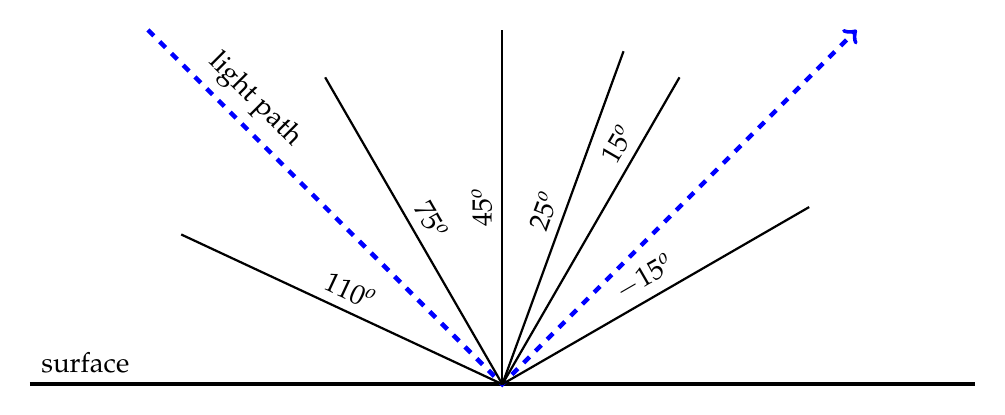
\begin{tikzpicture}[scale = 1.5]

\draw[ultra thick] (0, 0) node[above, anchor = south west] {surface} -- (8, 0) ;
\draw[dashed, ultra thick, ->, blue] (1, 3) -- (4, 0)
   node[black, near start, above, sloped] {light path} -- (7, 3);

\draw[thick] (0:4) -- node[above, near end, above, sloped] {\(15^o\)} +(60:3);
\draw[thick] (4, 0) -- node[above, midway, above, sloped] {\(25^o\)} +(70:3);
\draw[thick] (4, 0) -- node[above, midway, above, sloped] {\(45^o\)} +(90:3);
\draw[thick] (4, 0) -- node[above, midway, above, sloped] {\(75^o\)} +(120:3);
\draw[thick] (4, 0) -- node[above, midway, above, sloped] {\(110^o\)} +(155:3);
\draw[thick] (4, 0) -- node[above, midway, above, sloped] {\(-15^o\)} +(30:3);

\end{tikzpicture}
\end{verbatim}

\begin{center}
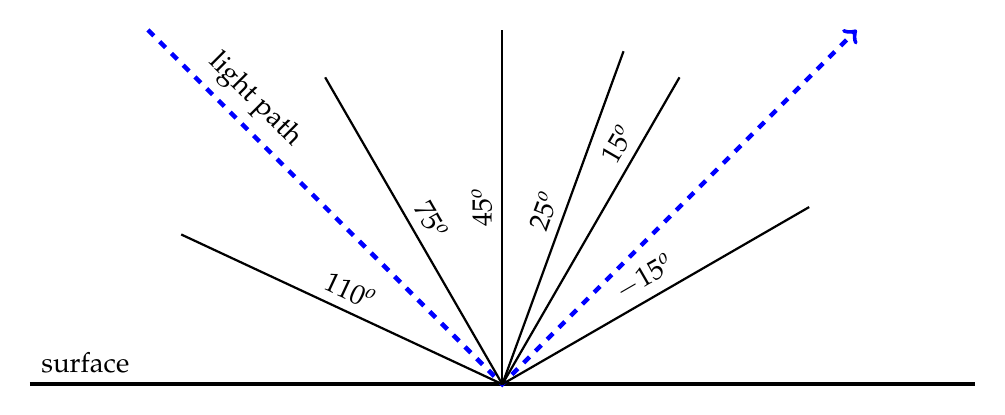
\begin{tikzpicture}[scale = 1.5]

\draw[ultra thick] (0, 0) node[above, anchor = south west] {surface} -- (8, 0) ;
\draw[dashed, ultra thick, ->, blue] (1, 3) -- (4, 0)
   node[black, near start, above, sloped] {light path} -- (7, 3);

\draw[thick] (0:4) -- node[above, near end, above, sloped] {\(15^o\)} +(60:3);
\draw[thick] (4, 0) -- node[above, midway, above, sloped] {\(25^o\)} +(70:3);
\draw[thick] (4, 0) -- node[above, midway, above, sloped] {\(45^o\)} +(90:3);
\draw[thick] (4, 0) -- node[above, midway, above, sloped] {\(75^o\)} +(120:3);
\draw[thick] (4, 0) -- node[above, midway, above, sloped] {\(110^o\)} +(155:3);
\draw[thick] (4, 0) -- node[above, midway, above, sloped] {\(-15^o\)} +(30:3);

\end{tikzpicture}
\end{center}

I don't use it to full force, but there's a \href{https://julien.danjou.info/projects/emacs-packages#org-contacts}{contributed Org-mode package} for managing
contacts. It stores details in a property drawer (added with \texttt{C-c C-x p}) like this:

\subsection*{Henderson, John}
\label{sec:orgheadline10}
\begin{verbatim}
Email: jw.hendy@gmail.com
Company: 3M
\end{verbatim}

You can integrate this with \texttt{gnus}, and email mode for Emacs. I have quite a bit of
trouble with this due to the work firewall, so I've not gone that far\ldots{} though I'd \emph{love} to
handle my emails in Emacs! I often copy/paste snippets from eamils into an Org-mode
journal tree so I don't have to keep things in my inbox anyway.

\section*{Example analysis}
\label{sec:orgheadline14}

For the last section, I want to go through how I typically set up experimental data
analyses, as well as commenting on some of the code-related features. My analyses are
typically on project-specific data as the result of some test or set of experiments. If
it's really quick, I'll just write things up in my main notes file and, if needed, export
just the subtree (we'll get to that).

If the experiment warrants some more serious analysis and a writeup/presentation, I'll often create a
dedicated folder for it. My structure tends to look like this:

\begin{verbatim}
tree --dirsfirst
\end{verbatim}

\begin{verbatim}
.
├── data
├── img
├── plots
└── demo_article.org

3 directories, 1 file
\end{verbatim}

Lately, I've been going through data from the same machine on different samples, which
can generate an awful lot of files. My preference has been to create a master file with
ids/data/file names of the samples, and then read the raw data into a list based on that
file. 

I typically use an initial block, set not to export, to do the preliminary
read-in/processing. This way, I run it once and then set to \texttt{:eval no} so it doesn't
re-run each export (the results are already in the R session).

\subsection*{Experimental results}
\label{sec:orgheadline12}

From here, I often generate a "prettier" plot for use in my report or presentation. I also
noticed an issue with \texttt{samp\_1\_1} when I generated it, so I'd opt to prune it as I think the
test data is suspect.

To use \texttt{:results output graphics}, you  have to specify an output file with \texttt{:file}. You
can keep lines shorter by adding as many \texttt{\#+header:} lines as you want (which supplements
the options passed after \texttt{\#+begin\_src}. You need a \texttt{\#+name} for the code block so that if
you change code and re-run, Org-mode knows to update the original results block vs. adding
one each time you execute.

You can add backend-specific formatting options to the results. Here is the default
generate Org-mode code to include results:

\begin{verbatim}
#+RESULTS: rate-compare
[[file:./plots/rate-comparison.png]]
\end{verbatim}

For PDF, I typically center and adjust size as desired:

\begin{verbatim}
#+begin_center
#+caption: Rate comparison of samples 1-4
#+attr_latex: :width 0.9\textwidth
#+attr_html: :width 75%
#+RESULTS: rate-compare
[[file:./plots/rate-comparison.png]]
#+end_center
\end{verbatim}

\begin{center}
\begin{figure}[htb]
\centering
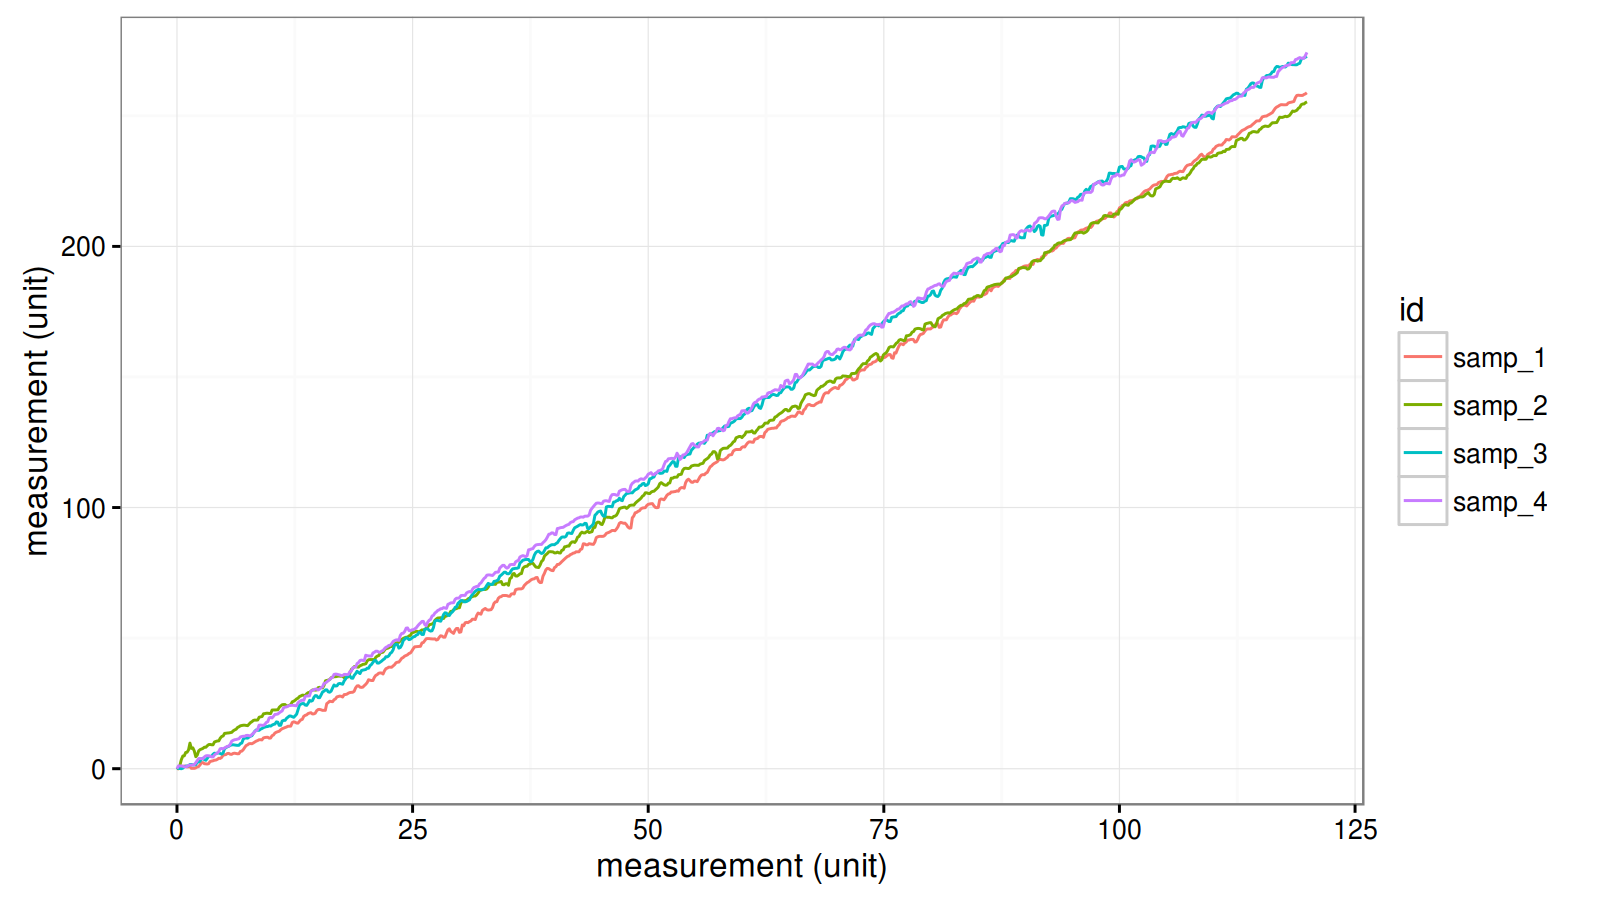
\includegraphics[width=0.9\textwidth]{./plots/rate-comparison.png}
\caption{Rate comparison of samples 1-4}
\end{figure}
\end{center}

I also quite enjoy the \texttt{ascii} package, as it has a mode to turn a data frame into
Org-mode table format:

\begin{verbatim}
stats <- stats[stats$grp != "samp_1_1", ]
stat_table <- ascii(stats, include.rownames = F,
              rownames = rep("", 6), colnames = names(stats))
print(stat_table)
\end{verbatim}

\begin{center}
\begin{tabular}{lrlrrrr}
\toprule
id & rep & grp & x\(_{\text{max}}\) & y\(_{\text{max}}\) & rate & delta\\
\midrule
samp\(_{\text{1}}\) & 2.00 & samp\(_{\text{1}}_{\text{2}}\) & 119.88 & 258.82 & 2.16 & 13.02\\
samp\(_{\text{2}}\) & 1.00 & samp\(_{\text{2}}_{\text{1}}\) & 119.90 & 255.33 & 2.13 & 16.23\\
samp\(_{\text{3}}\) & 1.00 & samp\(_{\text{3}}_{\text{1}}\) & 119.90 & 272.75 & 2.27 & 1.22\\
samp\(_{\text{4}}\) & 1.00 & samp\(_{\text{4}}_{\text{1}}\) & 119.90 & 274.27 & 2.29 & 0.00\\
\bottomrule
\end{tabular}
\end{center}

You can have \texttt{R} spit out Org-mode syntax as well, which is nice for repetitive
operations. You could process numerous text files and create a headline for each one. I
used this to input a \texttt{.csv} with budget data for 3M groups, outputting a reference cheat
sheet with account numbers and the next year's budget for each group chair in a separate
subtree. It's a little tedious (lots of \texttt{cat()} lines), but for \textasciitilde{}40 groups, it was well
worth it.

\subsection*{Conclusion}
\label{sec:orgheadline13}

That's it for the quick demo. You can copy these code blocks or results to any other
Org-mode file, which I find particularly useful when writing up a larger report but
needing to present a synopsis at a team meeting, for example. With thoughful path
definitions (or just going with absolute paths), you can often copy these with very
minimal adjustments (usually only the \texttt{:width} or \texttt{:height} options to the graphic, which
I'll often change with \texttt{M-x replace-string}.

While this was \texttt{R} focused, Org-mode supports a lot of \href{http://orgmode.org/worg/org-contrib/babel/languages.html}{languages}. I like that you can
intersperse them freely, and hand off data (or save to \texttt{.csv} with one, then
process/analyze with another). I've just started getting into \texttt{python}, and would like to
save myself a step by having Org-mode house my sensor reading \emph{and} my processing/plotting
rather than having them be separate steps.
\end{document}
